\begin{figure}[t]
    \centering
    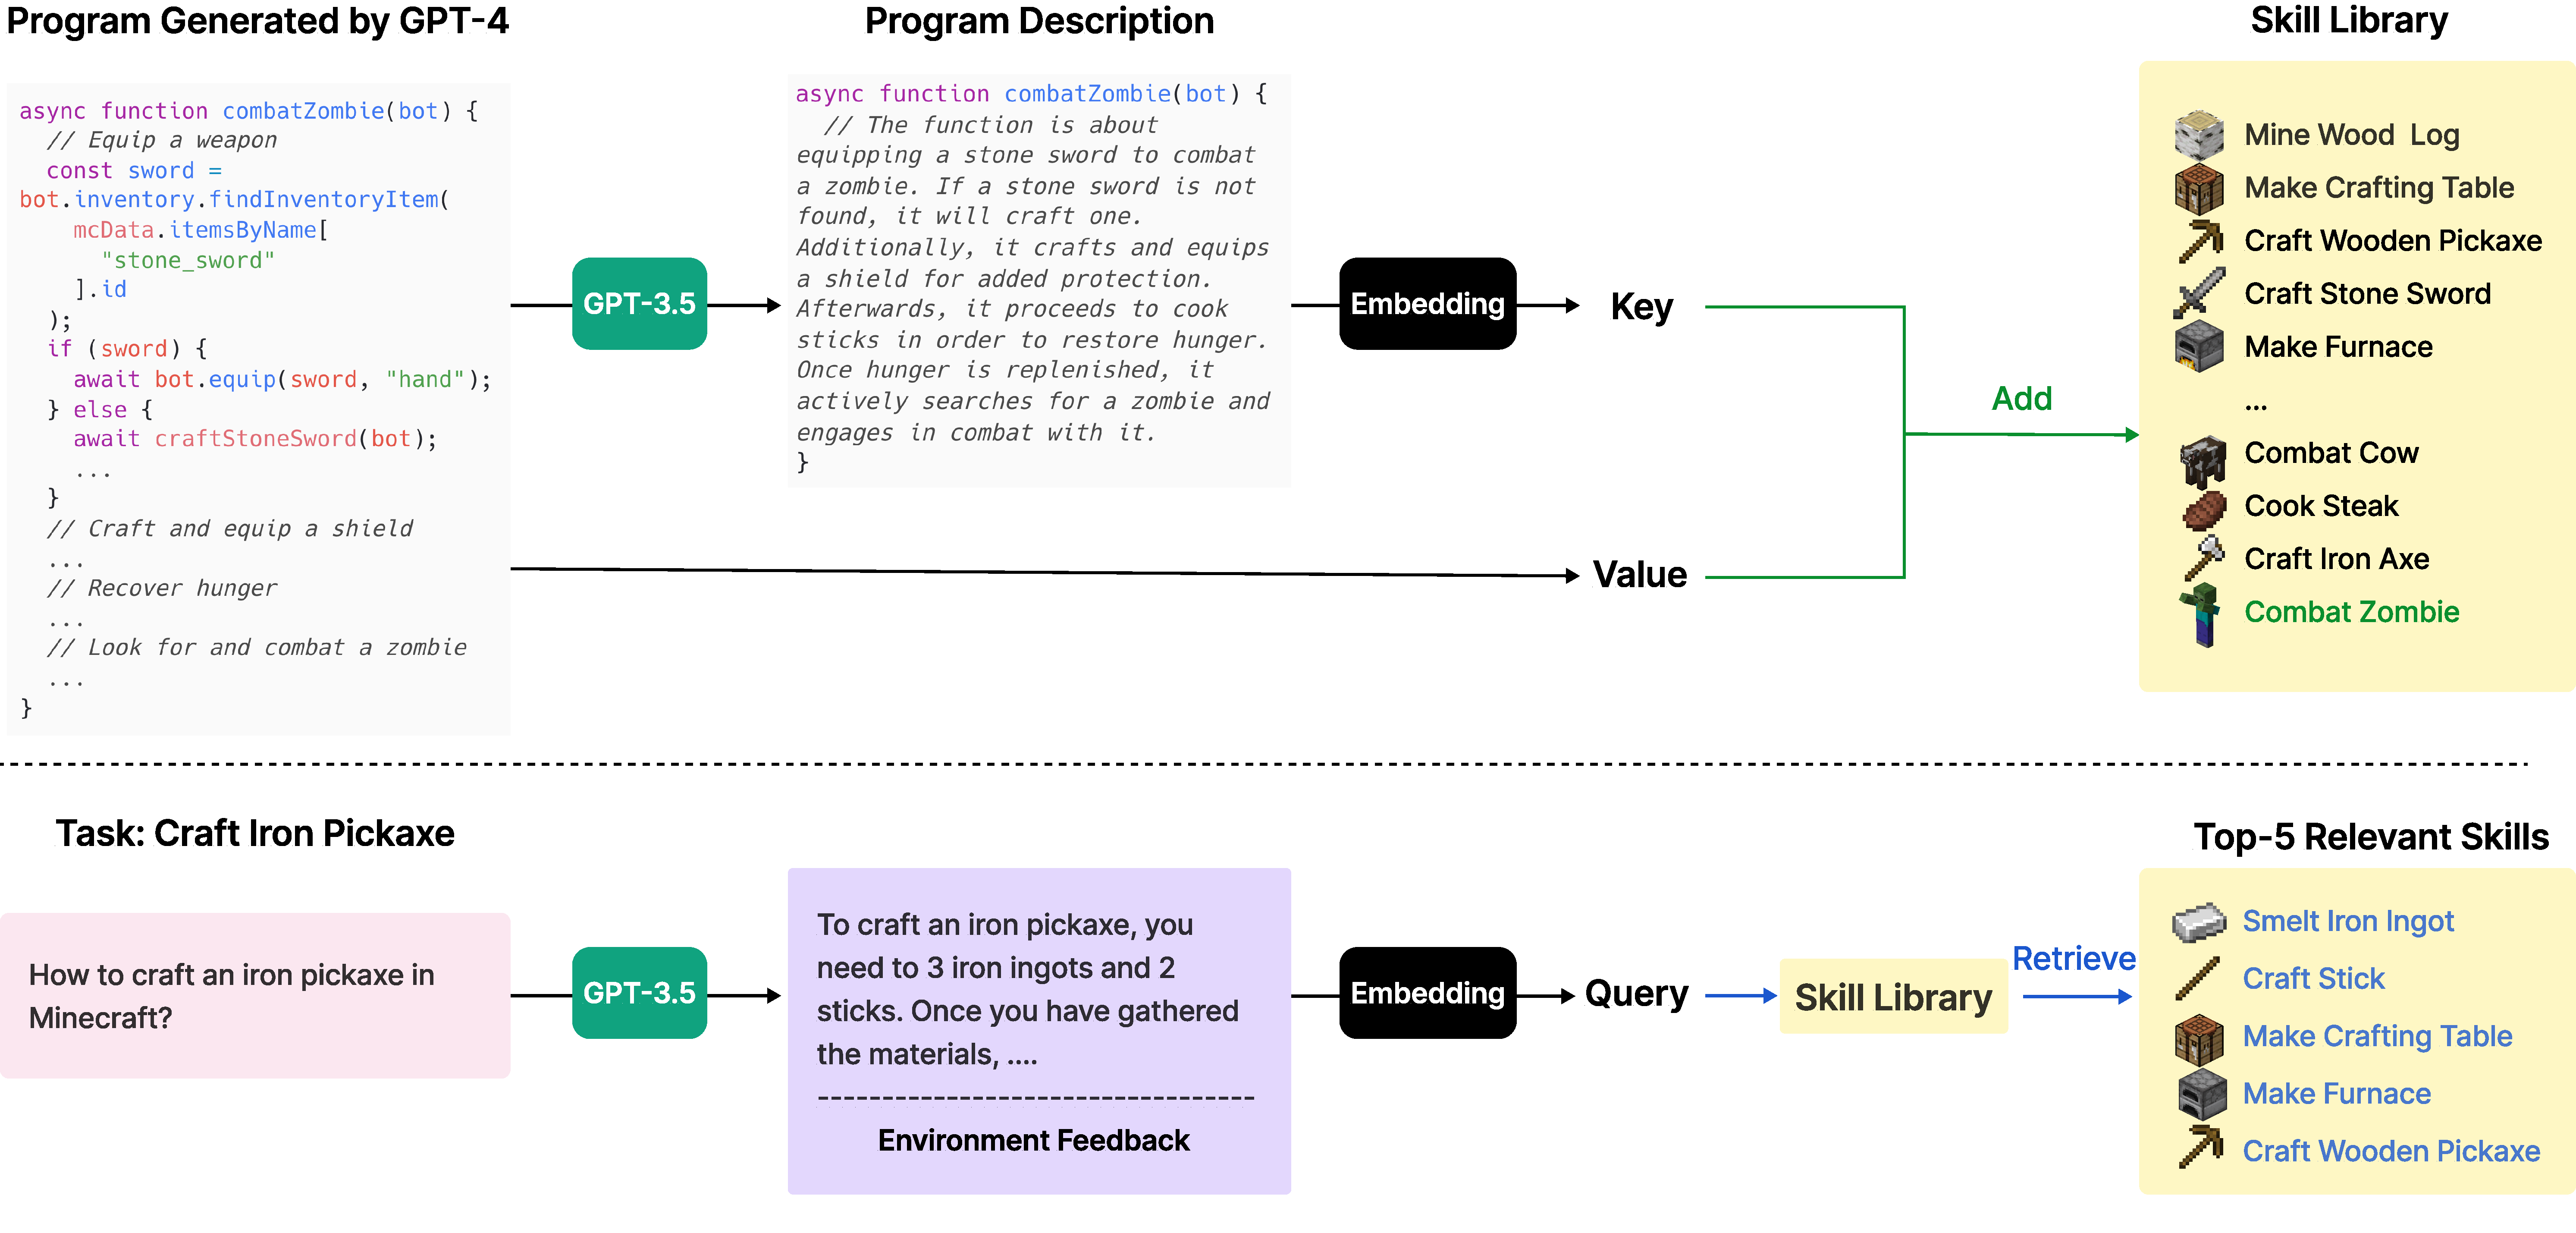
\includegraphics[width=\textwidth]{figures/skill_library_fig.pdf}
    \caption{
    \looseness=-1
    Skill library. \textbf{Top: Adding a new skill.} Each time GPT-4 generates and verifies a new skill, we add it to the skill library, represented by a vector database. The key is the embedding vector of the program description (generated by GPT-3.5), while the value is the program itself. \textbf{Bottom: Skill retrieval.} When faced with a new task proposed by the automatic curriculum, we first leverage GPT-3.5 to generate a general suggestion for solving the task, which is combined with environment feedback as the query context. Subsequently, we perform querying to identify the top-5 relevant skills.}
    \label{fig:skill_library}
    % \vspace{-1em}
\end{figure}